Primary author of this document: Andrew Groot \hypertarget{index_intro}{}\section{Introduction}\label{index_intro}
The \char`\"{}Wi-\/11 Machine\char`\"{} is a simple, 16-\/bit computer architecture. It has 8 general purpose registers, 3 condition code registers (CCRs), and a program counter (PC). The Wi-\/11 Simulator is meant to emulate its execution, as well as present the user with information regarding the state of the machine after each instruction is executed. However, before one can delve into the behind-\/the-\/scenes details, one must understand the environment. In particular, an understanding of the object file syntax and the interactions between the components used in this project is necessary.\hypertarget{index_syntax}{}\section{Object Files}\label{index_syntax}
\begin{DoxyParagraph}{}
The object files (usually file\_\-name.o) that this simulator accepts are ASCII text files with the following structure: \begin{DoxyItemize}
\item One \hyperlink{index_header}{Header Record} \item Zero or more \hyperlink{index_text}{Text Records} \item One \hyperlink{index_end}{End Record}\end{DoxyItemize}

\end{DoxyParagraph}
\hypertarget{index_header}{}\subsection{The Header Record}\label{index_header}
\begin{DoxyParagraph}{}
The Header Record is a single line that prepares the system for storing the instructions to come. 
\end{DoxyParagraph}
\begin{DoxyParagraph}{}
{\bfseries Components} \begin{DoxyItemize}
\item A capital 'H'. This designates that it is the Header Record. \item A 6 character \char`\"{}segment name\char`\"{} (anything will do). \item A 4-\/digit Hexadecimal value that corresponds to the \char`\"{}load address\char`\"{} of the program. Instructions can be written starting at this address. \item A second 4-\/digit Hexadecimal value that denotes the length of the program-\/load segment (the size of memory into which the instructions will be loaded). \end{DoxyItemize}

\end{DoxyParagraph}
\begin{DoxyParagraph}{}
{\bfseries At a glance:} There is an 'H', a segment name, the first location where instructions can be written, and the number of memory locations for instructions.
\end{DoxyParagraph}
\hypertarget{index_text}{}\subsection{Text Records}\label{index_text}
\begin{DoxyParagraph}{}
Following the Header Record are several Text Records. Each Text Record corresponds to a single machine instruction and, like the header record, is on a single line. 
\end{DoxyParagraph}
\begin{DoxyParagraph}{}
{\bfseries Components} \begin{DoxyItemize}
\item A capital 'T'. This designates that it is a Text Record. \item A 4-\/digit hexadecimal value -\/-\/ The location in memory at which the instruction will be stored. \item A second 4-\/digit Hexadecimal value -\/-\/ The encoding of the instruction to be stored. \end{DoxyItemize}

\end{DoxyParagraph}
\begin{DoxyParagraph}{}
{\bfseries At a glance:} There is a 'T', the location to store the instruction, and the instruction itself.
\end{DoxyParagraph}
\hypertarget{index_end}{}\subsection{The End Record}\label{index_end}
\begin{DoxyParagraph}{}
The End Record is, as the name would suggest, the last line of the file. Its purpose is to denote the end of instructions to be written and to give an initial value for the PC.\par
\par
 
\end{DoxyParagraph}
\begin{DoxyParagraph}{}
{\bfseries Components} \begin{DoxyItemize}
\item The End Record begins with a capital 'E'.\par
 \item Next, and last, a 4-\/digit hexadecimal value to be put into the PC. \end{DoxyItemize}

\end{DoxyParagraph}
\begin{DoxyParagraph}{}
{\bfseries At a glance:} There is an 'E', and the location in memory from which the first instruction should be fetched.
\end{DoxyParagraph}
\hypertarget{index_Component}{}\section{Interaction}\label{index_Component}
The components described in this document are, for the most part, representative of the actual hardware components that would be present in the Wi-\/11 machine. The following section describes these components and their interactions. After that, a list of the \hyperlink{index_instructions}{instructions} that the Wi-\/11 can execute (along with their encodings) completes the introduction to this simulator. The rest of the document details the workings of each component and provides the reader with the knowledge necessary for altering, fixing, or even just understanding the code itself.\hypertarget{index_components}{}\subsection{Components}\label{index_components}
The Wi-\/11 Simulator uses 5 major components (for a visual, see interactions). The main function, however, is only aware of one: \hyperlink{classWi11}{Wi11}. It creates one \hyperlink{classWi11}{Wi11} object and uses it to parse object files, decode the instructions, and execute them. In order to perform these tasks it first creates \hyperlink{classLoader}{Loader}, \hyperlink{classMemory}{Memory}, \hyperlink{classDecoder}{Decoder}, and \hyperlink{classRegister}{Register} objects. The \hyperlink{classRegister}{Register} objects correspond to all those mentioned in the \hyperlink{index_intro}{Introduction}, with the exception of the CCRs which are declared as their own entity.

\begin{DoxyNote}{Note}
The \hyperlink{classWord}{Word} class is not described below but nearly all transfers of data and mathematical operations are performed using (an) object(s) of this type.
\end{DoxyNote}
\hypertarget{index_loading}{}\subsubsection{Loading}\label{index_loading}
The \hyperlink{classLoader}{Loader} object, receiving a pointer to memory and a filename, creates an \hyperlink{classObjParser}{ObjParser} object (the fifth major component). The \hyperlink{classObjParser}{ObjParser} pulls the relevant data from the file and the \hyperlink{classLoader}{Loader} puts it into memory. After some input by the user is accepted (assuming the simulator is in debug mode), the \hyperlink{classWi11}{Wi11} is ready to begin executing instructions.\hypertarget{index_execution}{}\subsubsection{Executing}\label{index_execution}
The \hyperlink{classWi11}{Wi11} component executes instructions in a way very similar to how an actual Wi-\/11 machine would execute them. It first has the \hyperlink{classMemory}{Memory} object return the instruction referenced by the current value of the PC. After incrementing the PC, the raw instruction is given to the \hyperlink{classDecoder}{Decoder}. The \hyperlink{classDecoder}{Decoder} returns an \hyperlink{structInstruction}{Instruction} object that allows the \hyperlink{classWi11}{Wi11} to call one of its many private functions that correspond (one-\/to-\/one) to each kind of instruction. This process is then repeated until either the HALT trap code is found or the user-\/specified instruction limit is reached.


\begin{DoxyImage}
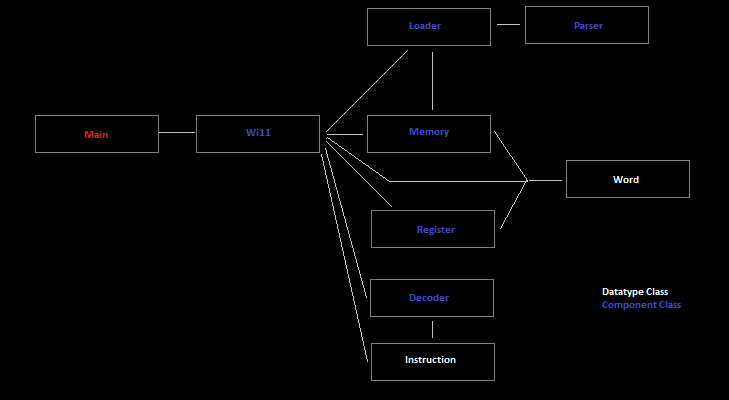
\includegraphics[width=\textwidth]{software_interaction.png}
\caption{This diagram shows the awareness of each component with those operating below it.}
\end{DoxyImage}
\hypertarget{index_instructions}{}\subsection{Wi-\/11 Instruction Set}\label{index_instructions}
\begin{DoxyParagraph}{}
This section describes the format of each operation on the Wi-\/11. First there are necessary definitions and then the list of instructions. The name of each instruction is followed by the opcode; this includes any base conversions that may be necessary. Then there is a list of the arguments to the command. The opcode is the first four bits of the instruction; the list following the opcode delegates purpose to the following 12 bits.
\end{DoxyParagraph}
\hypertarget{index_offset}{}\subsubsection{Offsets}\label{index_offset}
Offsets to the PC are used by concatenating them with the PC. Specifically, the first 7 bits of the PC and the 9 bit offset form the new PC value. This essentially separates memory into pages (the first seven bits of the PC corresponding a \char`\"{}page number\char`\"{}).\hypertarget{index_indexes}{}\subsubsection{Indexes}\label{index_indexes}
Indexes are used to specify a distance from a base value. Generally, there is a register holding an address. The index is added to the base address as a positive quantity (zero-\/extended) in order to form a new address. Because the index is zero-\/extended, the new address is always greater than the base address.\hypertarget{index_inst}{}\subsubsection{Intructions}\label{index_inst}
\begin{DoxyItemize}
\item ADD (two registers), OPCODE: 0001 (1) 
\begin{DoxyItemize}
\item 3 bits: The destination register 
\item 3 bits: First source register 
\item 1 bit: A zero 
\item 2 bits: Junk -\/ not used. 
\item 3 bits: Second source register 
\end{DoxyItemize}\item ADD (register and immediate), OPCODE: 0001 (1) 
\begin{DoxyItemize}
\item 3 bits: The destination register 
\item 3 bits: The source register 
\item 1 bit: A one 
\item 5 bits: An immediate value (2's complement) 
\end{DoxyItemize}\item AND (two registers), OPCODE: 0101 (5) 
\begin{DoxyItemize}
\item 3 bits: The destination register 
\item 3 bits: First source register 
\item 1 bit: A zero 
\item 2 bits: Junk -\/ not used 
\item 3 bits: Second source register 
\end{DoxyItemize}\item AND (register and immediate), OPCODE: 0101 (5) 
\begin{DoxyItemize}
\item 3 bits: The destination register 
\item 3 bits: The source register 
\item 1 bit: A one 
\item 5 bits: An immediate value (2's complement) 
\end{DoxyItemize}\item BRx, OPCODE: 0000 (0) 
\begin{DoxyItemize}
\item 1 bit: Corresponds to the CCR's negative bit 
\item 1 bit: Corresponds to the CCR's zero bit 
\item 1 bit: Corresponds to the CCR's positive bit 
\item 9-\/bits: An \hyperlink{index_offset}{offset} to the PC 
\end{DoxyItemize}\item DBUG, OPCODE: 1000 (8) 
\begin{DoxyItemize}
\item 12 bits: Junk -\/ not used 
\end{DoxyItemize}\item JSR, OPCODE: 0100 (4) 
\begin{DoxyItemize}
\item 1 bit: The link bit (The PC is stored in R7 if this is set) 
\item 2 bits: Junk -\/ not used 
\item 9 bits: An \hyperlink{index_offset}{offset} to the PC 
\end{DoxyItemize}\item JSRR, OPCODE: 1100 (12 -\/ C) 
\begin{DoxyItemize}
\item 1 bit: The link bit (The PC is stored in R7 if this is set) 
\item 2 bits: Junk -\/ not used 
\item 3 bits: A base register 
\item 6 bits: An \hyperlink{index_indexes}{index} to the base register 
\end{DoxyItemize}\item LD, OPCODE: 0010 (2) 
\begin{DoxyItemize}
\item 3 bits: The destination register 
\item 9 bits: An \hyperlink{index_offset}{offset} to the PC 
\end{DoxyItemize}\item LDI, OPCODE: 1010 (10 -\/ A) 
\begin{DoxyItemize}
\item 3 bits: The destination register 
\item 9 bits: An \hyperlink{index_offset}{offset} to the PC 
\end{DoxyItemize}\item LDR, OPCODE: 0110 (6) 
\begin{DoxyItemize}
\item 3 bits: The destination register 
\item 3 bits: A base register 
\item 6 bits: An \hyperlink{index_indexes}{index} to the base register 
\end{DoxyItemize}\item LEA, OPCODE: 1110 (14 -\/ E) 
\begin{DoxyItemize}
\item 3 bits: The destination register 
\item 9 bits: An \hyperlink{index_offset}{offset} to the PC 
\end{DoxyItemize}\item NOT, OPCODE: 1001 (9) 
\begin{DoxyItemize}
\item 3 bits: The destination register 
\item 3 bits: The source register 
\item 6 bits: Junk -\/ not used 
\end{DoxyItemize}\item RET, OPCODE: 1101 (13 -\/ D) 
\begin{DoxyItemize}
\item 12 bits: Junk -\/ not used 
\end{DoxyItemize}\item ST, OPCODE: 0011 (3) 
\begin{DoxyItemize}
\item 3 bits: The source register 
\item 9 bits: An \hyperlink{index_offset}{offset} to the PC 
\end{DoxyItemize}\item STI, OPCODE: 1011 (11 -\/ B) 
\begin{DoxyItemize}
\item 3 bits: The source register 
\item 9 bits: An \hyperlink{index_offset}{offset} to the PC 
\end{DoxyItemize}\item STR, OPCODE: 0111 (7) 
\begin{DoxyItemize}
\item 3 bits: The source register 
\item 3 bits: A base register 
\item 6 bits: An \hyperlink{index_indexes}{index} to the base register 
\end{DoxyItemize}\item TRAP, OPCODE: 1111 (15 -\/ F) 
\begin{DoxyItemize}
\item 4 bits: Junk -\/ not used 
\item 8 bits: A trap vector 
\end{DoxyItemize}\end{DoxyItemize}
\hypertarget{index_trap}{}\subsubsection{Traps}\label{index_trap}
Traps execute a system call. The details of these so-\/called \char`\"{}trap vectors\char`\"{} are below. \begin{DoxyItemize}
\item 0x21 -\/ OUT 
\begin{DoxyItemize}
\item Print the ASCII character in the last 8 bits of R0.
\end{DoxyItemize}\item 0x22 -\/ PUTS 
\begin{DoxyItemize}
\item Print the string starting at the address in R0 and ending at a null character.
\end{DoxyItemize}\item 0x23 -\/ IN 
\begin{DoxyItemize}
\item Prompt for and read an ASCII character. Put the result in R0.
\end{DoxyItemize}\item 0x25 -\/ HALT 
\begin{DoxyItemize}
\item End execution.
\end{DoxyItemize}\item 0x31 -\/ OUTN 
\begin{DoxyItemize}
\item Print the value in R0 as a decimal integer.
\end{DoxyItemize}\item 0x33 -\/ INN 
\begin{DoxyItemize}
\item Prompt for and read a decimal number. Put the result in R0.
\end{DoxyItemize}\item 0x43 -\/ RND 
\begin{DoxyItemize}
\item Generate a random integer and store it in R0.
\end{DoxyItemize}\end{DoxyItemize}
